
%<*visPLAIN>
% Use this tag to insert a blank page
\mbox{}
%</visPLAIN>

%<*vis01>
Enterprise Architect (EA) is a visual modelling tool that supports UML\footnote{Unified Modelling Language} and a host of other modelling languages.
EA is not only affordable but also quite flexible and can be extended via \emph{extensions} to support new modelling languages.
\begin{itemize}
\item[$\blacktriangleright$] Download EA for Windows from \url{http://www.sparxsystems.com/} to get a free 30 day trial and follow installation instructions (Fig.~\ref{fig_enterpriseArchitextHomepage}).

\begin{figure}[htbp]
	\centering
  	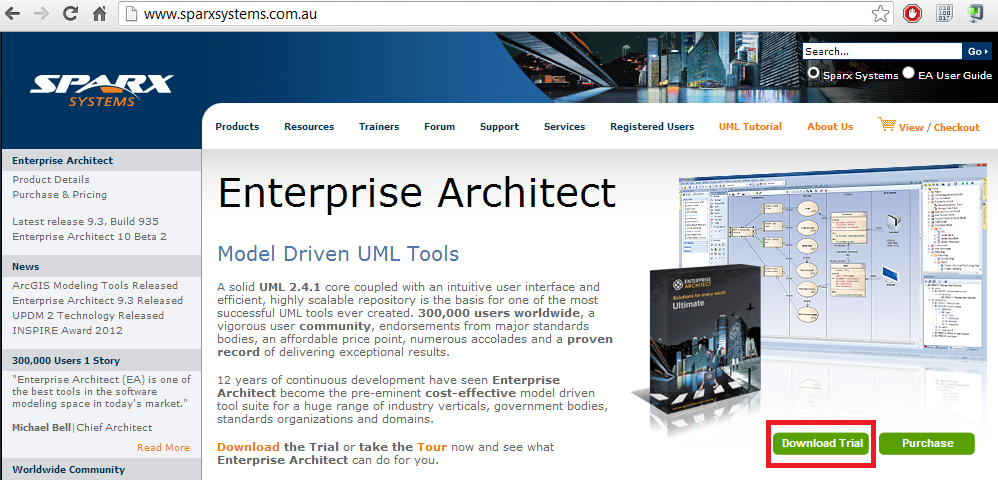
\includegraphics[width=0.77\textwidth]{ea_download}
	\caption{Download Enterprise Architect}
	\label{fig_enterpriseArchitextHomepage}
\end{figure} 

\item[$\blacktriangleright$] Install our EA-Extension (Fig.~\ref{fig_eaPluginWizard}) to add support for our modelling languages.
Download \url{http://www.moflon.org/fileadmin/download/moflon-ide/eclipse-plugin/ea-ecore-addin/ea-ecore-addin.zip}, unpack, and run \texttt{setup.exe}.

\begin{figure}[htbp]
	\centering
  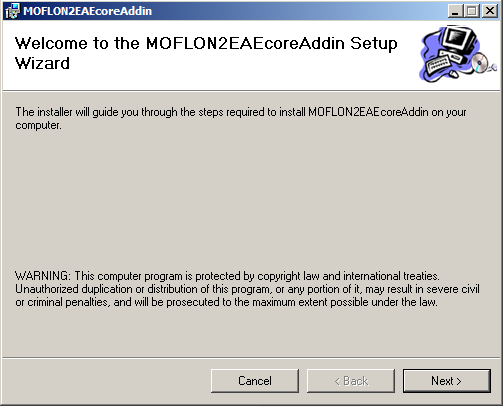
\includegraphics[width=0.55\textwidth]{eaplugin_install}
	\caption{Install our extension for EA}
	\label{fig_eaPluginWizard}
\end{figure}
\end{itemize}
%</vis01>



% Page 2
%<*vis02>
\begin{itemize}
\item[$\blacktriangleright$] In Eclipse, go to ``Window/Open Perspective/Other\ldots''\footnote{A path given as ``foo/bar'' indicates how to navigate in a series of menus and submenus.} and choose Moflon~(Fig.~\ref{fig_eclipse}).

\begin{figure}[htbp]
	\centering
  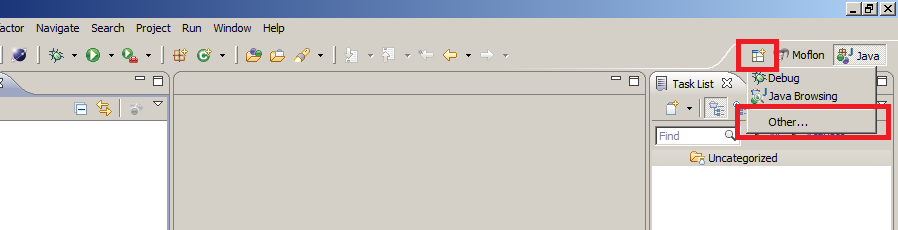
\includegraphics[width=\textwidth]{eclipse_firststart}
	\caption{Choose the Moflon perspective.}
	\label{fig_eclipse}
\end{figure} 

\item[$\blacktriangleright$] In the toolbar, a new action set should have appeared. Choose ``New Metamodel'' (Fig.~\ref{fig_eclipseNewMetamodel}).
The button with an ``L" shows you our logfile (important input for us if something goes wrong!).

\begin{figure}[htbp]
	\centering
  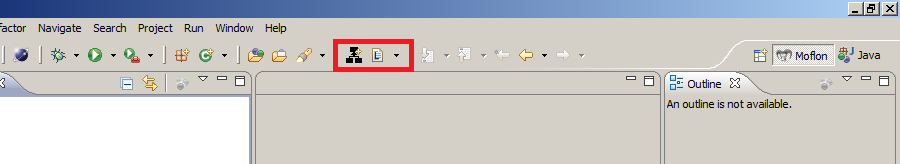
\includegraphics[width=\textwidth]{eclipse_metamodelButton}
	\caption{Eclipse ''New Metamodel''}
	\label{fig_eclipseNewMetamodel}
\end{figure}
 
\item[$\blacktriangleright$] Name the project 'Demo' and select 'Visual (Enterprise Architect)' . Make sure that the 'Add Demo Specification' is checked off. Press finish, and notice the Demo.eap file in your project explorer. This is the EA file you'll be testing and modelling your program with.
\\
\\
Please do not rename, move, or delete anything.

\end{itemize}
%</vis02>



%<*vis03>
\begin{itemize}
\FloatBarrier
% THIS NEEDS AN IMAGE
\item[$\blacktriangleright$] Press the small arrow in the package explorer, and choose working sets as your top level element (Fig.~\ref{fig_eclipseWorkingsets}). We work a lot with working sets, and use them to structure the workspace in Eclipse.

\item[$\blacktriangleright$] Double click ``Demo.eap'' to start EA, and choose ``Ultimate" when starting EA for the first time.

\item[$\blacktriangleright$] In EA, choose ``Extensions/MOFLON::Ecore Addin/Export\- all\- to\- Workspace'' (Fig.~\ref{fig_ea}).
You can of course browse the project structure, but please do not rename, move, or delete anything yet.

\begin{figure}[htbp]
	\centering
  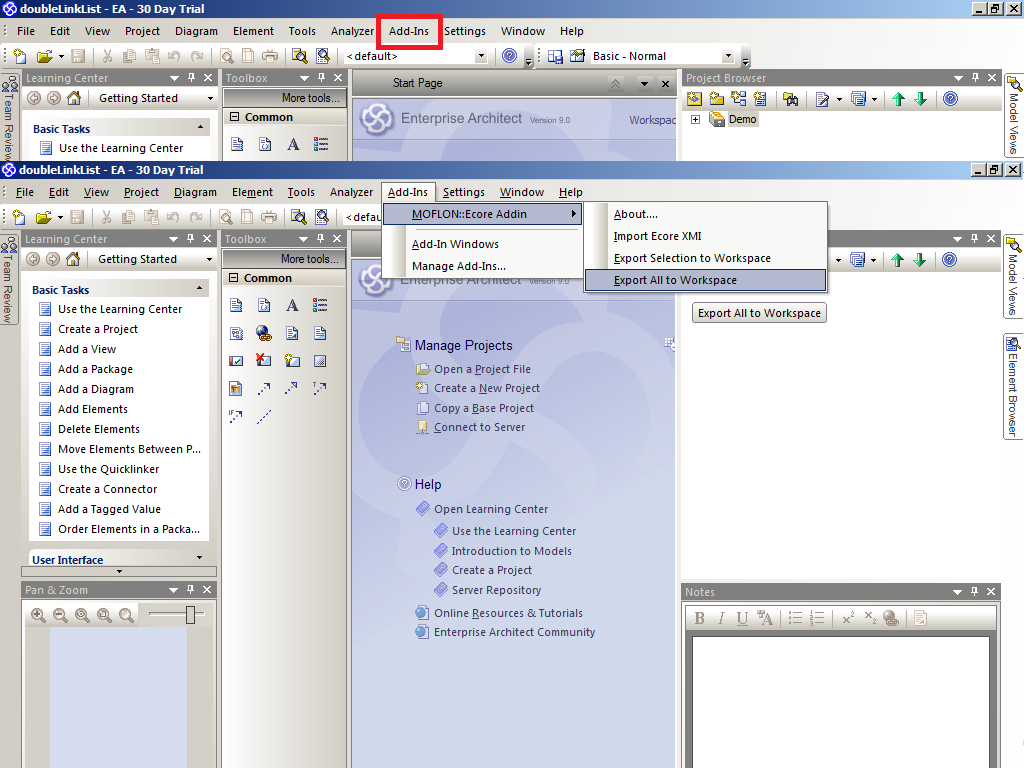
\includegraphics[width=0.9\textwidth]{ea_firststart}
	\caption{Export from EA using our extension} 
	\label{fig_ea} 
\end{figure}
  
\item[$\blacktriangleright$] Switch back to Eclipse, choose your Metamodel project, and press F5 to refresh.
The export from EA places all required files in a hidden folder in the project, and refreshing triggers a build process that invokes our code generators automatically.
You should be able to monitor the progress in the lower right corner (Fig.~\ref{fig_eclipsebuilding}).  
Pressing the symbol opens a monitor view that gives more details of the build process. 
You don't need to worry about any of these details, just remember to refresh your Eclipse workspace after an export.

\begin{figure}[htbp]
	\centering
  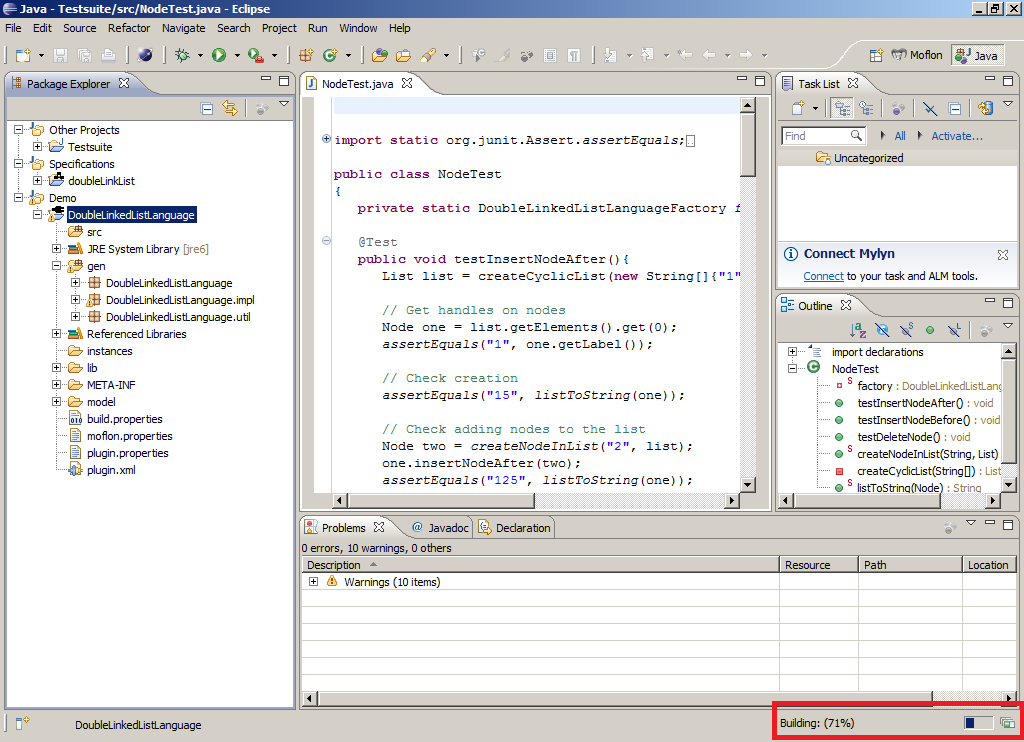
\includegraphics[width=0.55\textwidth]{eclipse_building}
	\caption{Automatically building the workspace after a refresh.}
	\label{fig_eclipsebuilding}
\end{figure}
\end{itemize}
%</vis03>